\begin{frame}
	\frametitle{The Big Bang}
	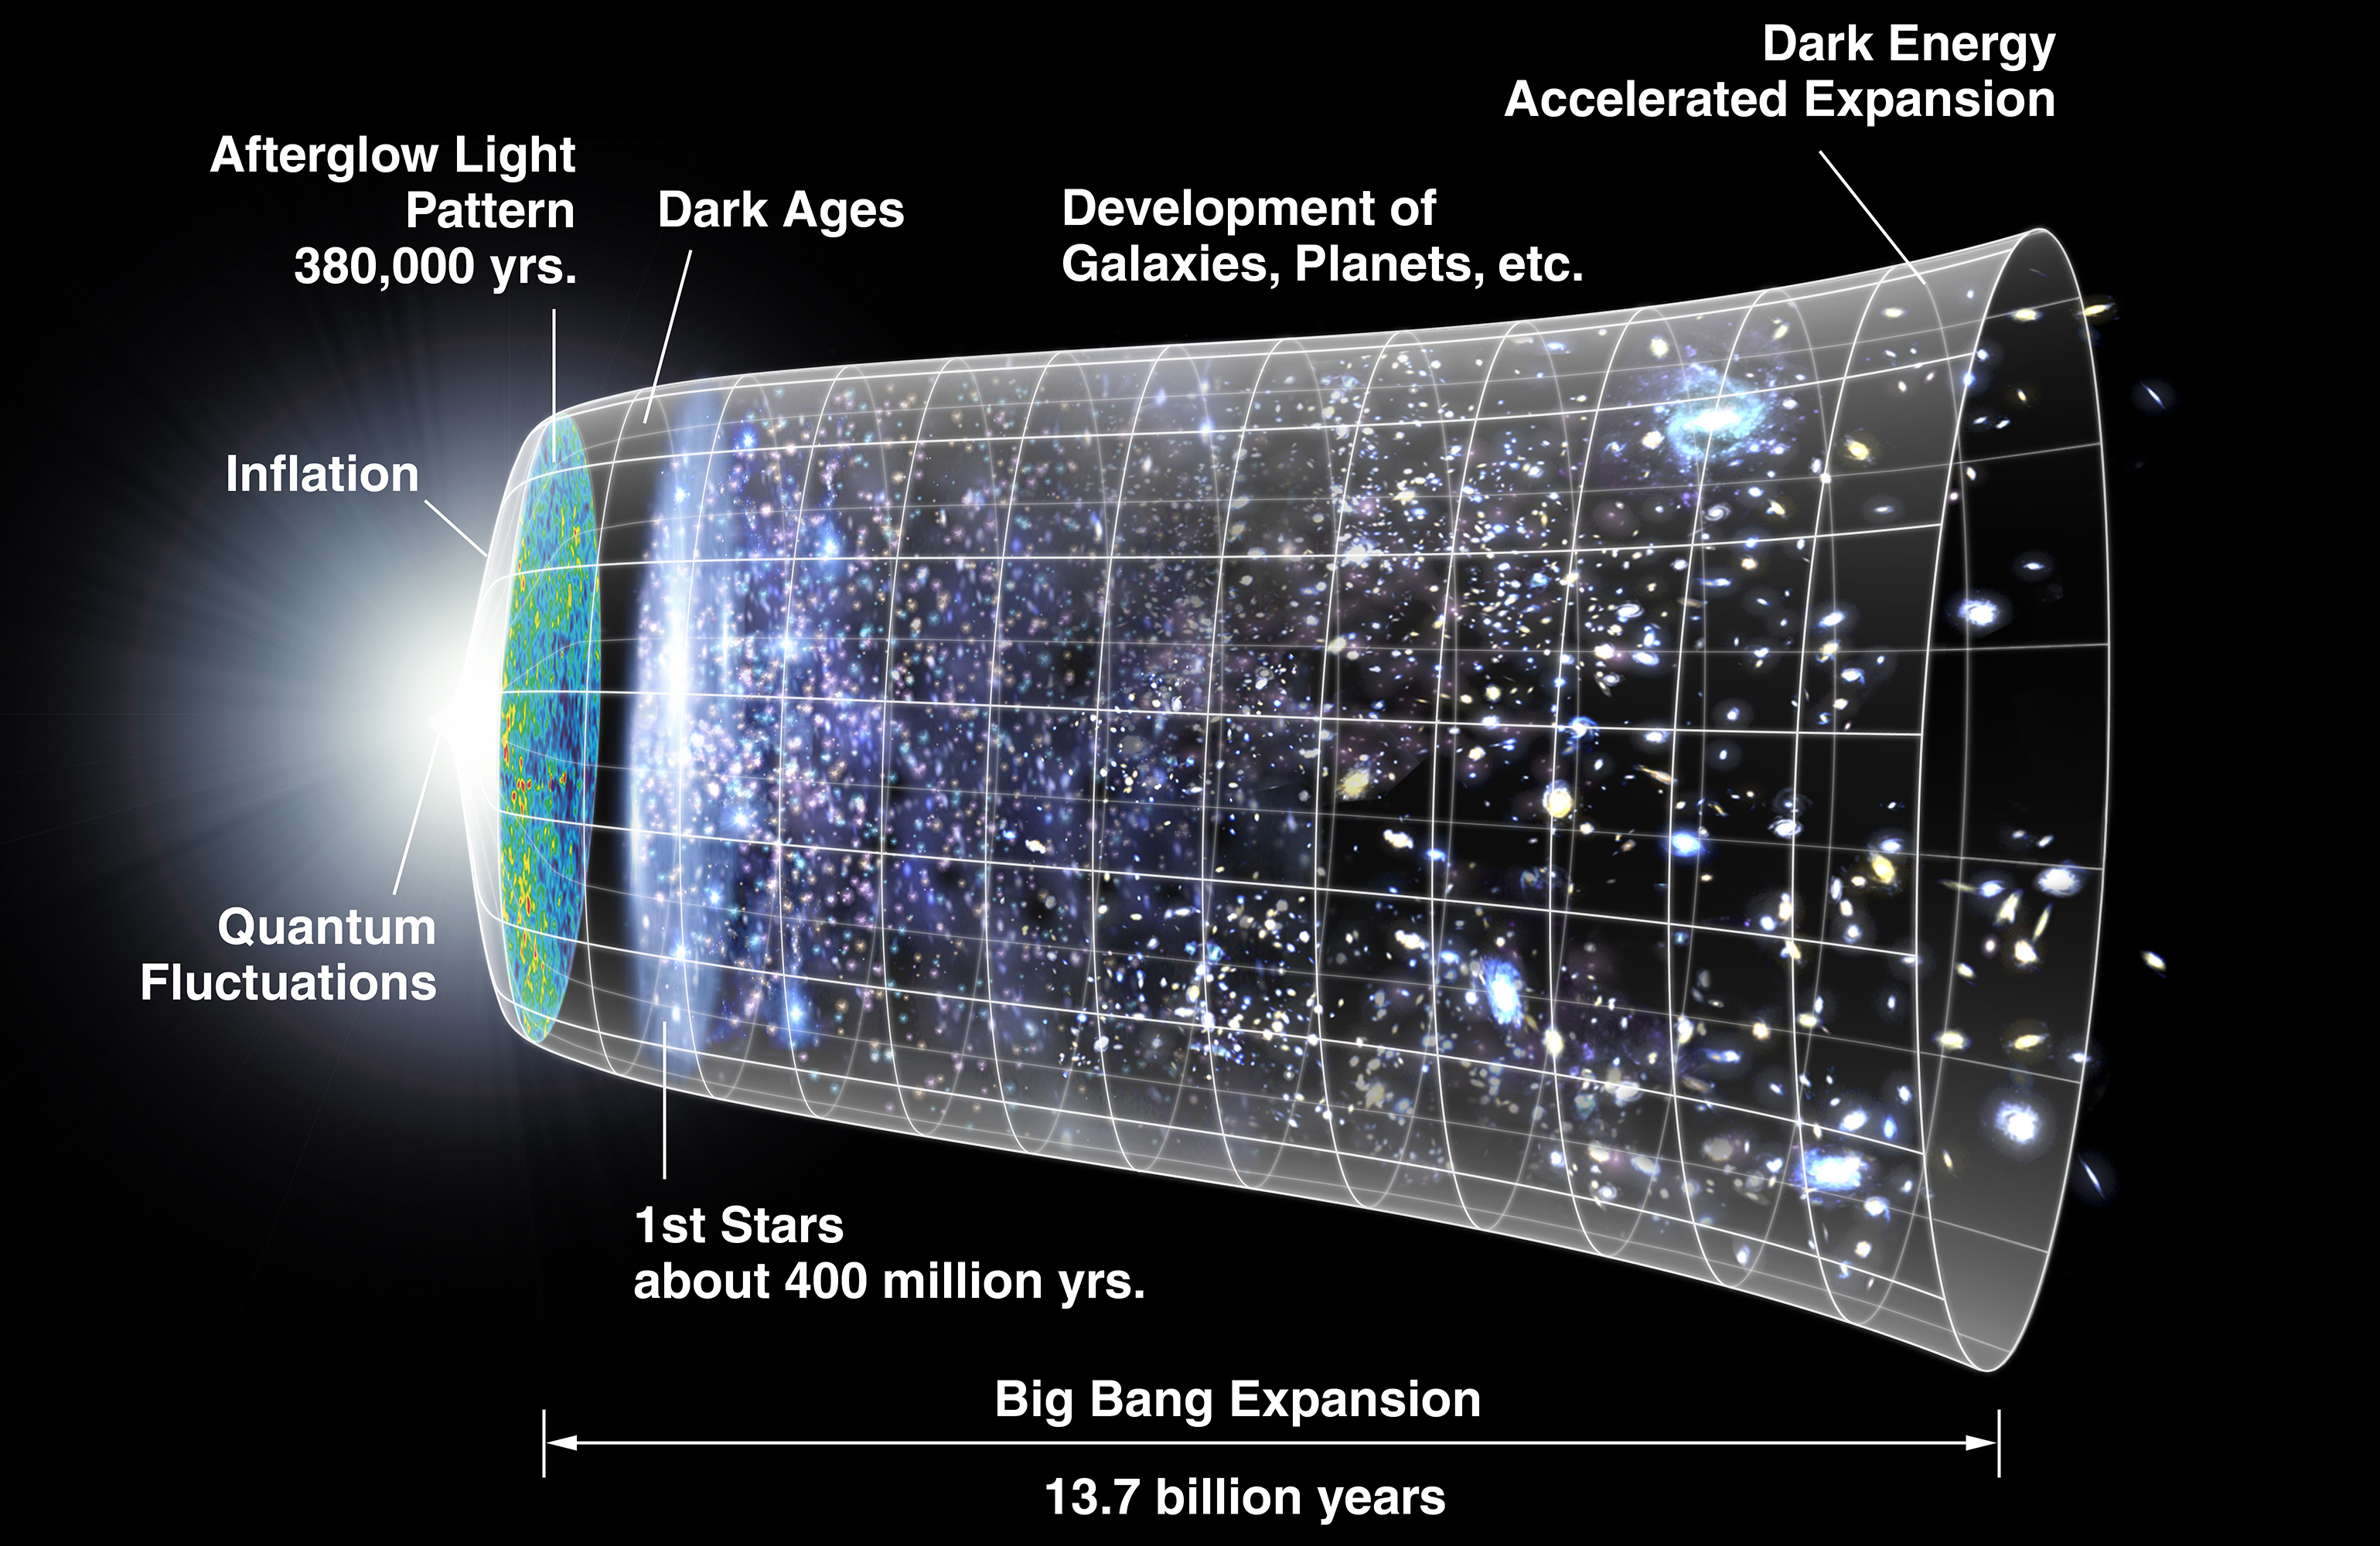
\includegraphics[width=\textwidth]{Images/Big_Bang.jpg}
\end{frame}

\begin{frame}
	\frametitle{The Big Bang}
	\framesubtitle{Evidence}

	There are two fundamental observations which led to the first Big Bang Theory being hypothesised and confirmed:

	\begin{itemize}
		\pause\item Galactic Redshifts
		\pause\item The Cosmic Microwave Background Radiation
	\end{itemize}
	
\end{frame}

\begin{frameb}{w}{Images/HubbleXDF.png}
	\frametitle{The Big Bang}
	\framesubtitle{Galactic Redshift}
\end{frameb}

\begin{frame}
	\frametitle{The Big Bang}
	\framesubtitle{Galactic Redshift}
	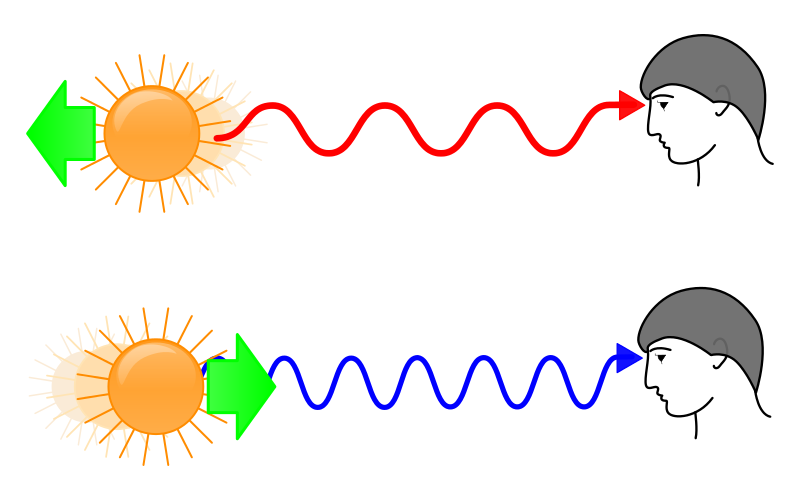
\includegraphics[width=\textwidth]{Images/redshift.png}
\end{frame}

\begin{frame}
	\frametitle{The Big Bang}
	\framesubtitle{Galactic Redshift}

	As observed by Edwin Hubble in 1929,
	it appears that:

	\begin{enumerate}
		\pause\item All Galaxies are moving away from us
		\pause\item The Further away they are, the faster they are moving away
		\pause\item If we were to go to another galaxy, we would see exactly the same thing
	\end{enumerate}

\end{frame}

\begin{frame}
	\frametitle{The Big Bang}
	\framesubtitle{A stretching universe:}
	\centerline{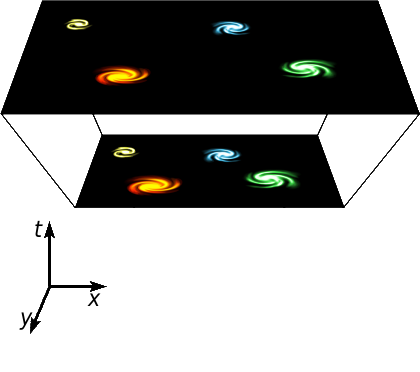
\includegraphics[height=0.8\textheight]{Images/Universe_expansion1.png}}
\end{frame}
\begin{frame}
	\frametitle{The Big Bang}
	\framesubtitle{A stretching universe:}
	\centerline{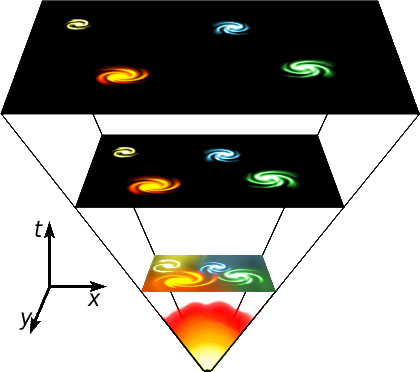
\includegraphics[height=0.8\textheight]{Images/Universe_expansion.png}}
\end{frame}

\begin{frame}
	\frametitle{The Big Bang}
	\framesubtitle{The Cosmic Microwave Background Radiation}
	\begin{columns}
	\begin{column}{0.5\textwidth}
		\begin{itemize}
			\item<1-> Discovered by accident in 1964 by Penzias \& Wilson.
			\item<2-> Experimenting with a supersensitive detector.
		\end{itemize}
	\end{column}
	\begin{column}{0.5\textwidth}
		\includegraphics<1->[width=\textwidth]{Images/penzias_wilson.jpg}
	\end{column}

	\end{columns}
	\vspace{0.5cm}

	\begin{itemize}
		\item<3-> Thermal radiation fills the universe at a temperature $T\approx3K$
		\item<4-> This is best explained as an `afterglow' of the Big Bang.
	\end{itemize}
\end{frame}


\begin{frame}
	\frametitle{The Big Bang}
	\framesubtitle{Common Misconceptions}
	The Big Bang does {\em NOT} look like this:
	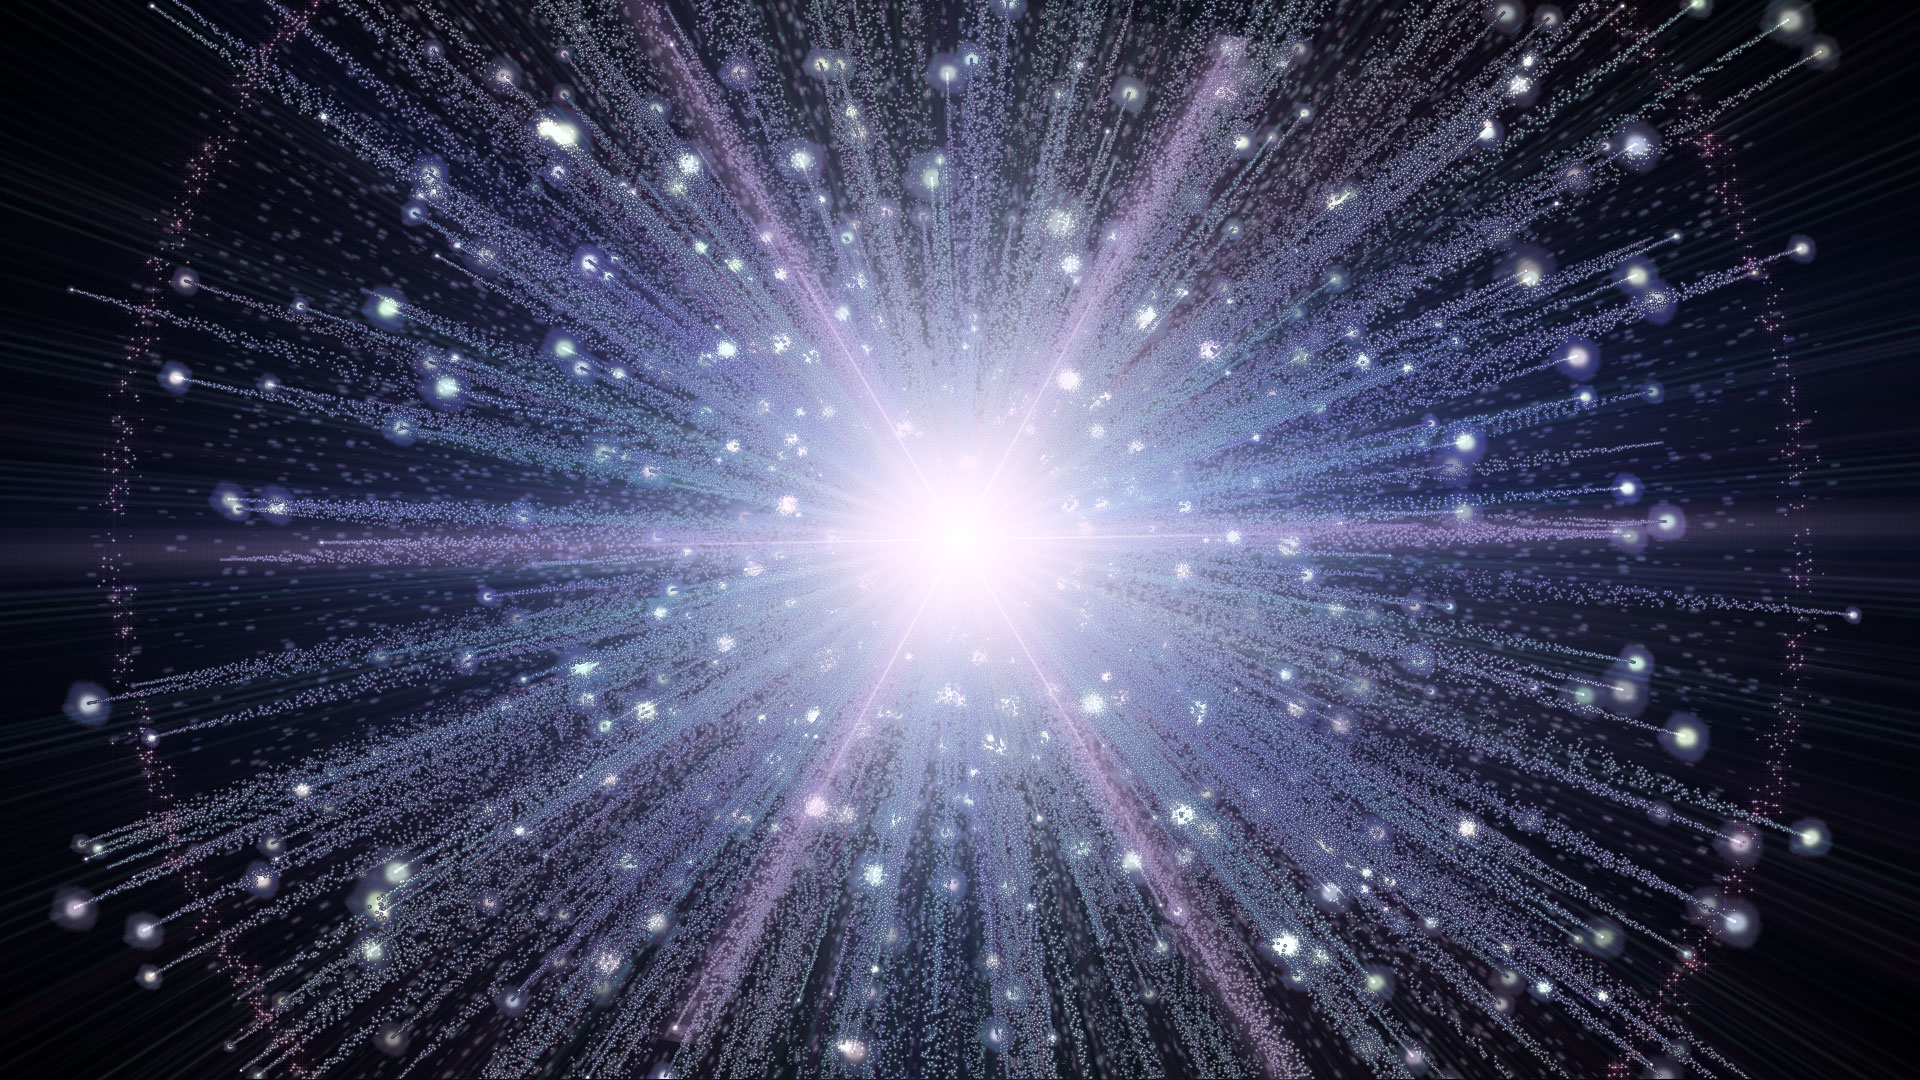
\includegraphics[width=\textwidth]{Images/bigbangnot.jpg}
	
\end{frame}

\begin{frame}
	\frametitle{The Big Bang}
	\framesubtitle{Common Misconceptions}

	\begin{itemize}
		\item Despite the name, the Big Bang is not an explosion.
		\pause\item The Universe is not necessarily expanding into anything.
	\end{itemize}
	
\end{frame}



